\usepackage{tikz}
    
\definecolor{accessibilitytag}{RGB}{202,161,241}
\tikzstyle{accessibilitytag} = [draw=accessibilitytag, fill=accessibilitytag, very thick, rectangle, rounded corners, inner sep=1pt, inner ysep=2pt]
\newcommand{\accessibilitytag}{
\begin{tikzpicture}\node [accessibilitytag] (box){{\scriptsize \color{white}{\textbf{\phantom{|}a11y\phantom{|}}}}};\end{tikzpicture}}
\usepackage{tikz}
    
\definecolor{amazonsthreetag}{RGB}{0,134,194}
\tikzstyle{amazonsthreetag} = [draw=amazonsthreetag, fill=amazonsthreetag, very thick, rectangle, rounded corners, inner sep=1pt, inner ysep=2pt]
\newcommand{\amazonsthreetag}{
\begin{tikzpicture}\node [amazonsthreetag] (box){{\scriptsize \color{white}{\textbf{\phantom{|}Amazon S3\phantom{|}}}}};\end{tikzpicture}}
\usepackage{tikz}
    
\definecolor{androidtag}{RGB}{167,224,130}
\tikzstyle{androidtag} = [draw=androidtag, fill=androidtag, very thick, rectangle, rounded corners, inner sep=1pt, inner ysep=2pt]
\newcommand{\androidtag}{
\begin{tikzpicture}\node [androidtag] (box){{\scriptsize \textbf{\phantom{|}Android\phantom{|}}}};\end{tikzpicture}}
\usepackage{tikz}
    
\definecolor{apitag}{RGB}{234,234,134}
\tikzstyle{apitag} = [draw=apitag, fill=apitag, very thick, rectangle, rounded corners, inner sep=1pt, inner ysep=2pt]
\newcommand{\apitag}{
\begin{tikzpicture}\node [apitag] (box){{\scriptsize \textbf{\phantom{|}API\phantom{|}}}};\end{tikzpicture}}
\usepackage{tikz}
    
\definecolor{backbonetag}{RGB}{0,134,194}
\tikzstyle{backbonetag} = [draw=backbonetag, fill=backbonetag, very thick, rectangle, rounded corners, inner sep=1pt, inner ysep=2pt]
\newcommand{\backbonetag}{
\begin{tikzpicture}\node [backbonetag] (box){{\scriptsize \color{white}{\textbf{\phantom{|}BackboneJS\phantom{|}}}}};\end{tikzpicture}}
\usepackage{tikz}
    
\definecolor{cicdtag}{RGB}{124,186,112}
\tikzstyle{cicdtag} = [draw=cicdtag, fill=cicdtag, very thick, rectangle, rounded corners, inner sep=1pt, inner ysep=2pt]
\newcommand{\cicdtag}{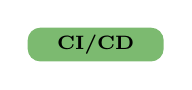
\begin{tikzpicture}\node [cicdtag] (box){{\scriptsize \textbf{\phantom{|}CI/CD\phantom{|}}}};\end{tikzpicture}}
\usepackage{tikz}
    
\definecolor{circlecitag}{RGB}{70,189,64}
\tikzstyle{circlecitag} = [draw=circlecitag, fill=circlecitag, very thick, rectangle, rounded corners, inner sep=1pt, inner ysep=2pt]
\newcommand{\circlecitag}{
\begin{tikzpicture}\node [circlecitag] (box){{\scriptsize \textbf{\phantom{|}CircleCI\phantom{|}}}};\end{tikzpicture}}
\usepackage{tikz}
    
\definecolor{csstag}{RGB}{40,168,221}
\tikzstyle{csstag} = [draw=csstag, fill=csstag, very thick, rectangle, rounded corners, inner sep=1pt, inner ysep=2pt]
\newcommand{\csstag}{
\begin{tikzpicture}\node [csstag] (box){{\scriptsize \textbf{\phantom{|}CSS\phantom{|}}}};\end{tikzpicture}}
\usepackage{tikz}
    
\definecolor{djangotag}{RGB}{12,60,38}
\tikzstyle{djangotag} = [draw=djangotag, fill=djangotag, very thick, rectangle, rounded corners, inner sep=1pt, inner ysep=2pt]
\newcommand{\djangotag}{
\begin{tikzpicture}\node [djangotag] (box){{\scriptsize \color{white}{\textbf{\phantom{|}Django\phantom{|}}}}};\end{tikzpicture}}
\usepackage{tikz}
    
\definecolor{eclipseplugintag}{RGB}{157,146,240}
\tikzstyle{eclipseplugintag} = [draw=eclipseplugintag, fill=eclipseplugintag, very thick, rectangle, rounded corners, inner sep=1pt, inner ysep=2pt]
\newcommand{\eclipseplugintag}{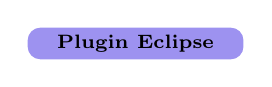
\begin{tikzpicture}\node [eclipseplugintag] (box){{\scriptsize \textbf{\phantom{|}Plugin Eclipse\phantom{|}}}};\end{tikzpicture}}
\usepackage{tikz}
    
\definecolor{emberjstag}{RGB}{224,78,57}
\tikzstyle{emberjstag} = [draw=emberjstag, fill=emberjstag, very thick, rectangle, rounded corners, inner sep=1pt, inner ysep=2pt]
\newcommand{\emberjstag}{
\begin{tikzpicture}\node [emberjstag] (box){{\scriptsize \color{white}{\textbf{\phantom{|}EmberJS\phantom{|}}}}};\end{tikzpicture}}
\usepackage{tikz}
    
\definecolor{estag}{RGB}{207,207,207}
\tikzstyle{estag} = [draw=estag, fill=estag, very thick, rectangle, rounded corners, inner sep=1pt, inner ysep=2pt]
\newcommand{\estag}{
\begin{tikzpicture}\node [estag] (box){{\scriptsize \textbf{\phantom{|}ElasticSearch\phantom{|}}}};\end{tikzpicture}}
\usepackage{tikz}
    
\definecolor{gatsbytag}{RGB}{101,51,149}
\tikzstyle{gatsbytag} = [draw=gatsbytag, fill=gatsbytag, very thick, rectangle, rounded corners, inner sep=1pt, inner ysep=2pt]
\newcommand{\gatsbytag}{
\begin{tikzpicture}\node [gatsbytag] (box){{\scriptsize \color{white}{\textbf{\phantom{|}Gatsby\phantom{|}}}}};\end{tikzpicture}}
\usepackage{tikz}
    
\definecolor{gcptag}{RGB}{0,134,194}
\tikzstyle{gcptag} = [draw=gcptag, fill=gcptag, very thick, rectangle, rounded corners, inner sep=1pt, inner ysep=2pt]
\newcommand{\gcptag}{
\begin{tikzpicture}\node [gcptag] (box){{\scriptsize \color{white}{\textbf{\phantom{|}GCP\phantom{|}}}}};\end{tikzpicture}}
\usepackage{tikz}
    
\definecolor{githubactionstag}{RGB}{246,186,53}
\tikzstyle{githubactionstag} = [draw=githubactionstag, fill=githubactionstag, very thick, rectangle, rounded corners, inner sep=1pt, inner ysep=2pt]
\newcommand{\githubactionstag}{
\begin{tikzpicture}\node [githubactionstag] (box){{\scriptsize \textbf{\phantom{|}Github Actions\phantom{|}}}};\end{tikzpicture}}
\usepackage{tikz}
    
\definecolor{hibernatetag}{RGB}{188,174,121}
\tikzstyle{hibernatetag} = [draw=hibernatetag, fill=hibernatetag, very thick, rectangle, rounded corners, inner sep=1pt, inner ysep=2pt]
\newcommand{\hibernatetag}{
\begin{tikzpicture}\node [hibernatetag] (box){{\scriptsize \textbf{\phantom{|}Hibernate\phantom{|}}}};\end{tikzpicture}}
\usepackage{tikz}
    
\definecolor{internationalizationtag}{RGB}{161,202,241}
\tikzstyle{internationalizationtag} = [draw=internationalizationtag, fill=internationalizationtag, very thick, rectangle, rounded corners, inner sep=1pt, inner ysep=2pt]
\newcommand{\internationalizationtag}{
\begin{tikzpicture}\node [internationalizationtag] (box){{\scriptsize \color{white}{\textbf{\phantom{|}i18n\phantom{|}}}}};\end{tikzpicture}}
\usepackage{tikz}
    
\definecolor{iostag}{RGB}{215,134,234}
\tikzstyle{iostag} = [draw=iostag, fill=iostag, very thick, rectangle, rounded corners, inner sep=1pt, inner ysep=2pt]
\newcommand{\iostag}{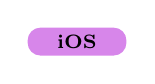
\begin{tikzpicture}\node [iostag] (box){{\scriptsize \textbf{\phantom{|}iOS\phantom{|}}}};\end{tikzpicture}}
\usepackage{tikz}
    
\definecolor{javatag}{RGB}{234,144,144}
\tikzstyle{javatag} = [draw=javatag, fill=javatag, very thick, rectangle, rounded corners, inner sep=1pt, inner ysep=2pt]
\newcommand{\javatag}{
\begin{tikzpicture}\node [javatag] (box){{\scriptsize \textbf{\phantom{|}Java\phantom{|}}}};\end{tikzpicture}}
\usepackage{tikz}
    
\definecolor{jstag}{RGB}{248,220,61}
\tikzstyle{jstag} = [draw=jstag, fill=jstag, very thick, rectangle, rounded corners, inner sep=1pt, inner ysep=2pt]
\newcommand{\jstag}{
\begin{tikzpicture}\node [jstag] (box){{\scriptsize \color{darkgray}{\textbf{\phantom{|}JS\phantom{|}}}}};\end{tikzpicture}}
\usepackage{tikz}
    
\definecolor{kubernetestag}{RGB}{0,134,194}
\tikzstyle{kubernetestag} = [draw=kubernetestag, fill=kubernetestag, very thick, rectangle, rounded corners, inner sep=1pt, inner ysep=2pt]
\newcommand{\kubernetestag}{
\begin{tikzpicture}\node [kubernetestag] (box){{\scriptsize \color{white}{\textbf{\phantom{|}Kubernetes\phantom{|}}}}};\end{tikzpicture}}
\usepackage{tikz}
    
\definecolor{lesstag}{RGB}{29,53,92}
\tikzstyle{lesstag} = [draw=lesstag, fill=lesstag, very thick, rectangle, rounded corners, inner sep=1pt, inner ysep=2pt]
\newcommand{\lesstag}{
\begin{tikzpicture}\node [lesstag] (box){{\scriptsize \color{white}{\textbf{\phantom{|}LESS\phantom{|}}}}};\end{tikzpicture}}
\usepackage{tikz}
    
\definecolor{lotusnotestag}{RGB}{246,186,53}
\tikzstyle{lotusnotestag} = [draw=lotusnotestag, fill=lotusnotestag, very thick, rectangle, rounded corners, inner sep=1pt, inner ysep=2pt]
\newcommand{\lotusnotestag}{
\begin{tikzpicture}\node [lotusnotestag] (box){{\scriptsize \textbf{\phantom{|}Lotus Notes\phantom{|}}}};\end{tikzpicture}}
\usepackage{tikz}
    
\definecolor{nodejstag}{RGB}{2,88,0}
\tikzstyle{nodejstag} = [draw=nodejstag, fill=nodejstag, very thick, rectangle, rounded corners, inner sep=1pt, inner ysep=2pt]
\newcommand{\nodejstag}{
\begin{tikzpicture}\node [nodejstag] (box){{\scriptsize \color{white}{\textbf{\phantom{|}Node.js\phantom{|}}}}};\end{tikzpicture}}
\usepackage{tikz}
    
\definecolor{objectivectag}{RGB}{134,206,234}
\tikzstyle{objectivectag} = [draw=objectivectag, fill=objectivectag, very thick, rectangle, rounded corners, inner sep=1pt, inner ysep=2pt]
\newcommand{\objectivectag}{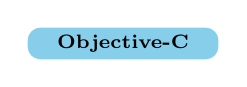
\begin{tikzpicture}\node [objectivectag] (box){{\scriptsize \textbf{\phantom{|}Objective-C\phantom{|}}}};\end{tikzpicture}}
\usepackage{tikz}
    
\definecolor{pythontag}{RGB}{55,118,171}
\tikzstyle{pythontag} = [draw=pythontag, fill=pythontag, very thick, rectangle, rounded corners, inner sep=1pt, inner ysep=2pt]
\newcommand{\pythontag}{
\begin{tikzpicture}\node [pythontag] (box){{\scriptsize \textbf{\phantom{|}Python\phantom{|}}}};\end{tikzpicture}}
\usepackage{tikz}
    
\definecolor{reacttag}{RGB}{95,217,251}
\tikzstyle{reacttag} = [draw=reacttag, fill=reacttag, very thick, rectangle, rounded corners, inner sep=1pt, inner ysep=2pt]
\newcommand{\reacttag}{
\begin{tikzpicture}\node [reacttag] (box){{\scriptsize \textbf{\phantom{|}React\phantom{|}}}};\end{tikzpicture}}
\usepackage{tikz}
    
\definecolor{sasstag}{RGB}{204,102,153}
\tikzstyle{sasstag} = [draw=sasstag, fill=sasstag, very thick, rectangle, rounded corners, inner sep=1pt, inner ysep=2pt]
\newcommand{\sasstag}{
\begin{tikzpicture}\node [sasstag] (box){{\scriptsize \textbf{\phantom{|}SASS\phantom{|}}}};\end{tikzpicture}}
\usepackage{tikz}
    
\definecolor{springtag}{RGB}{124,186,112}
\tikzstyle{springtag} = [draw=springtag, fill=springtag, very thick, rectangle, rounded corners, inner sep=1pt, inner ysep=2pt]
\newcommand{\springtag}{
\begin{tikzpicture}\node [springtag] (box){{\scriptsize \textbf{\phantom{|}Spring\phantom{|}}}};\end{tikzpicture}}
\usepackage{tikz}
    
\definecolor{sqlitetag}{RGB}{234,175,230}
\tikzstyle{sqlitetag} = [draw=sqlitetag, fill=sqlitetag, very thick, rectangle, rounded corners, inner sep=1pt, inner ysep=2pt]
\newcommand{\sqlitetag}{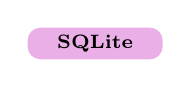
\begin{tikzpicture}\node [sqlitetag] (box){{\scriptsize \textbf{\phantom{|}SQLite\phantom{|}}}};\end{tikzpicture}}
\usepackage{tikz}
    
\definecolor{stenciljstag}{RGB}{224,78,57}
\tikzstyle{stenciljstag} = [draw=stenciljstag, fill=stenciljstag, very thick, rectangle, rounded corners, inner sep=1pt, inner ysep=2pt]
\newcommand{\stenciljstag}{
\begin{tikzpicture}\node [stenciljstag] (box){{\scriptsize \textbf{\phantom{|}StencilJS\phantom{|}}}};\end{tikzpicture}}
\usepackage{tikz}
    
\definecolor{terraformtag}{RGB}{109,103,230}
\tikzstyle{terraformtag} = [draw=terraformtag, fill=terraformtag, very thick, rectangle, rounded corners, inner sep=1pt, inner ysep=2pt]
\newcommand{\terraformtag}{
\begin{tikzpicture}\node [terraformtag] (box){{\scriptsize \color{white}{\textbf{\phantom{|}Terraform\phantom{|}}}}};\end{tikzpicture}}
\usepackage{tikz}
    
\definecolor{vuejstag}{RGB}{53,148,105}
\tikzstyle{vuejstag} = [draw=vuejstag, fill=vuejstag, very thick, rectangle, rounded corners, inner sep=1pt, inner ysep=2pt]
\newcommand{\vuejstag}{
\begin{tikzpicture}\node [vuejstag] (box){{\scriptsize \color{white}{\textbf{\phantom{|}Vue.js\phantom{|}}}}};\end{tikzpicture}}
\usepackage{tikz}
    
\definecolor{websockettag}{RGB}{234,175,230}
\tikzstyle{websockettag} = [draw=websockettag, fill=websockettag, very thick, rectangle, rounded corners, inner sep=1pt, inner ysep=2pt]
\newcommand{\websockettag}{
\begin{tikzpicture}\node [websockettag] (box){{\scriptsize \textbf{\phantom{|}WebSocket\phantom{|}}}};\end{tikzpicture}}
